\section{Thesis Organisation}
\label{sec:introduction:organisation}

We organise the thesis into four parts. \textbf{\Cref{part:preface}~(\textit{The Preface})} includes introductory, background and methodology chapters. This is a \textit{PhD by Publication}, and \textbf{\cref{part:publications}~(\textit{Publications})} comprises of seven publications resulting from this work over \Cref{ch:icsme2019,ch:tse2020,ch:icse2020,ch:fse-demo2020,ch:fse2020,ch:icwe2019,ch:semotion2020}; publications are included verbatim except for terminology and formatting changes to better fit the suitability of a coherent thesis. \textbf{\Cref{part:postface}~(\textit{The Postface})} includes the conclusion and future works chapter, as well as a list of academic studies and online artefacts referenced within the thesis. \textbf{\Cref{part:appendices}~(\textit{Appendices})} includes all supplementary material, including mandatory authorship statements and ethics approval. Details of each chapter following this introductory chapter are provided in the following section.

\subsection{\Cref{part:preface}: Preface}

\subsubsection{\cref{ch:background}: Background} This chapter provides an overview of prior studies broadly around three key pillars: the development of an \gls{iws}, the usage of an \gls{iws}, and the nature of an \gls{iws}. We use the three perspectives of software quality (particularly, reliability), probabilistic and non-deterministic systems, and explanation and communication theory to describe prior work.

\subsubsection{\cref{ch:research-methodology}: Research Methodology} This chapter provides a summative review of research methods and philosophical stances relevant to \glslong{se}. We illustrate that the methods used within our publications are sound via an analysis of the methodologies used in seminal works referenced in this thesis.

\subsection{\Cref{part:publications}: Publications}

\subsubsection{\cref{ch:icsme2019}: Exploring the nature of \glspl{cvs}} This chapter was presented at the 2019 International Conference on Software Maintenance and Evolution~(ICSME)~\citep{Cummaudo:2019icsme}. We describe an 11-month longitudinal experiment assessing the behavioural (run-time) issues of three popular \glspl{cvs}: Google Cloud Vision~\citepweb{GoogleCloud:Home}, Amazon Rekognition~\citepweb{AWS:Home} and Azure Computer Vision~\citepweb{Azure:Home}. By using three different data sets---two of which we curate as additional contributions---we demonstrate how the services are inconsistent amongst each other and within themselves. This study provides a detailed answer to \ref{rq:nature}: Despite presenting conceptually-similar functionality, each service behaves and produces slightly varied (inconsistent) results and demonstrates non-deterministic runtime behaviour. We discuss potential evolution risks to consumers of such services as the services provide non-static outputs for the same inputs, thereby having significant impact to the robustness of consuming applications. Further details in the study include a brief assessment into the lack of sufficient detail of these concerns in their documentation.

\subsubsection{\cref{ch:icse2020}: Understanding developer struggles when using \glspl{cvs}} This chapter has been accepted for presentation at the 2020 International Conference on Software Engineering~(ICSE)~\citep{Cummaudo:2020icse}. We conduct a mining study of 1,425 \glslong{so} questions that provide indications of the types frustrations that developers face when integrating \glspl{cvs} into their applications. To gather what their pain-points are, we use two classification taxonomies that also use \glslong{so} to understand generalised and documentation-specific pain-points in mature \gls{se} domains. This study answers \ref{rq:devs} in detail and provides a validation to our motivation of \ref{rq:docs}: we validate that the \textit{completeness} of current \gls{cvs} \gls{api} documentation is a main concern for developers and there is insufficient explanation into the errors and limitations of the service. We find that the documentation does not adequately cover all aspects of the technical domain. In terms of integrating with the service, developers struggle most with simple errors and ways in which to use the \glspl{api}; this is in stark contrast to mature software domains. Our interpretation is that developers fail to understand the \gls{iws} lifecycle and the `whole' system that wraps such services. We also interpret that developers have a shallower understanding of the core issues within \glspl{cvs} (likely due to the nuances of \gls{ml} as suggested in a discussion in the paper), which warrants an avenue for future work in \glslong{se} education.

\subsubsection{\cref{ch:semotion2020}: Ranking \gls{cvs} pain-points by frustration} This chapter has been submitted to the the 2020 International Workshop on Emotion Awareness in Software Engineering (SEmotion)~\citep{Curumsing:2020semotion}. In this work, we use our dataset consisting of the 1,425 \gls{so} questions from \citep{Cummaudo:2020icse} to interpret the breakdown of emotions developers express per classification of pain-points conducted in \cref{ch:icse2020}. We find that the distribution of various emotions differ per question type, and developers are most frustrated when the expectations of a \gls{cvs} does not match the reality of what these services actually provide, which shapes our answer for \ref{rq:devs:frustration} and thus \ref{rq:devs}.

\subsubsection{\cref{ch:tse2020}: Investigating improvements to \gls{cvs} \gls{api} documentation} This chapter was originally a short paper presented at the 2019 International Symposium on Empirical Software Engineering and Measurement~(ESEM) \citep{Cummaudo:2020icse}. To understand where to improve \gls{cvs} documentation, we first need to investigate \textit{what} makes a good \gls{api} document. This short paper initially answered one aspect of \ref{rq:docs:complete}: what \textit{academic literature} suggests a good (complete) \gls{api} document should comprise of. By conducting an \glslong{sms} resulting in 21 primary studies, we systematically develop a taxonomy that combines the recommendations of scattered work into a structured framework of 5 dimensions and 34 weighted categorisations. We then extend this work by triangulating the taxonomy with opinions from developers using the \glslong{sus} to assess the efficacy of these recommendations (thereby answering the second aspect of \ref{rq:docs:complete}). From this, we assess the how well \gls{cvs} providers document their \glspl{api} via a heuristic validation of the taxonomy, using the three services from the ICSME publication to make recommendations where documentation should be more complete, thereby answering \ref{rq:docs:missing} (and thus \ref{rq:docs}). The extended version of this chapter has been submitted to the IEEE Transactions on Software Engineering (TSE) in~\citep{Cummaudo:2020tse} and is currently in review.

\subsubsection{\cref{ch:icwe2019}: Merging responses of multiple \glspl{cvs}} This chapter was presented at the 2019 International Conference on Web Engineering~(ICWE)~\citep{Ohtake:2019vi}. Early exploration of \glspl{cvs} showed that multiple services use vastly different ontologies for the same input. As an initial strategy to improve the reliability of these services, we explored if merging multiple responses using WordNet \citep{WordNetMiller1995} and a novel label merging algorithm based on the proportional representation approach used in political voting could make any improvements. While this approach resulted in a modest improvement to reliability, it did not consider to the evolution issues or developer pain-points we later identified.

\subsubsection{\cref{ch:fse-demo2020}: Developing a confidence thresholding tool} This chapter has been submitted to the demonstrations track at FSE 2020~\citep{Cummaudo:2020fse-demo}. When integrating with a \gls{cvs}, developers need to select an appropriate confidence threshold suited to their use case and determine whether a decision should be made. An issue, however, is that these \glspl{cvs} are not calibrated to the specific problem-domain datasets and it is difficult for software developers to determine an appropriate confidence threshold on their problem domain. This tool presents a workflow and supporting tool for application developers to select decision thresholds suited to their domain that---unlike existing tooling---is designed to be used in pre-development, pre-release and production. This tooling forms part of a solution to \ref{rq:design} for developers to maintain robustness and reliability in their systems.

\subsubsection{\cref{ch:fse2020}: Developing a \gls{cvs} integration architecture} This chapter has been submitted to the 2020 Joint European Software Engineering Conference and Symposium on the Foundations of Software Engineering~\citep{Cummaudo:2020fse}. \todo[Based on the findings, we propose a set of new service error codes for describing the empirically observed error conditions of \gls{iws} based on our findings in \cref{ch:icsme2019}. To achieve this, we propose a proxy server intermediary that lies between a client application and a \gls{iws}; the proxy server tactic is designed to return these error codes when substantial evolution occurs against a benchmark dataset that represents the application domain context (similar to that proposed in \cref{ch:fse-demo2020}). A technical evaluation of our implementation of this architecture identifies 1,054 cases of substantial evolution in confidence values and 2,461 cases of evolution in the response label sets when 331 images were sent to a \gls{cvs}.]{AC: Added findings from this paper}

\subsection{\Cref{part:postface}: Postface}

In \Cref{ch:conclusions}, we review the contributions made in this thesis and the relevance and significance to identifying and resolving key issues when application developers integrate with \gls{cvs}. We evaluate these outcomes with reference to the research goals, and discuss threats to validity of the work. Lastly, we discuss the various avenues of research arising from this work. References from literature and a list of online artefacts are provided after this concluding chapter.

\subsection{\Cref{part:appendices}: Appendices}

\Cref{ch:additional-materials} provides additional material referenced within this thesis but not provided in the body. The source code for the reference architecture described in \cref{ch:fse2020} is reproduced in \cref{ch:reference-architecture-code}. The supplementary materials published with \cref{ch:tse2020} are reproduced in \cref{ch:tse-supplementary-materials}, which also describes the list of primary sources arising in the \glslong{sms} we conducted.
 We provide mandatory coauthor declaration forms describing the contribution breakdown for each publication within \cref{ch:authorship-statements}. \Cref{ch:ethics} contains copies of the ethics clearance for various experiments within this thesis. 

\begin{table}
  \centering
  \caption[List of publications resulting from this thesis]{List of publications resulting from this thesis, separated by phenomena exploration (above) and solution design (below).}
  \label{tab:introduction:structure:list-of-pubs}
  \tablefit{\begin{tabular}{rp{0.4\linewidth}ccc|cc}
    \toprule
    \textbf{Ref.} &
    \textbf{Venue} &
    \textbf{Acronym} &
    \textbf{Rank\tablefootnote{Conference publications ranking measured using the CORE Conference Ranks (\url{http://www.core.edu.au/conference-portal}) and Journal publications rankings using the Scimago Ranking (\url{https://www.scimagojr.com/}). Rankings retrieved January 2020.}} &
    \textbf{Published\tablefootnote{Date of publication, if applicable.}} &
    \textbf{Chapter} &
    \textbf{RQs}\\
    \midrule
    
    % ICSME
    \citep{Cummaudo:2019icsme} &
    35\textsuperscript{th} International Conference on Software Maintenance and Evolution &
    ICSME &
    A &
    05 Dec 2019 &
    \cref{ch:icsme2019} &
    \ref{rq:nature} \\

    % ESEM
    \citep{Cummaudo:2019esem} &
    13\textsuperscript{th} International Symposium on Empirical Software Engineering and Measurement &
    ESEM &
    A &
    17 Oct 2019 &
    Excluded\tablefootnote{The extended version of this conference proceeding is provided in \cref{ch:tse2020}.} &
    \ref{rq:docs:complete} \\
    
    % ICSE
    \citep{Cummaudo:2020icse}&
    42\textsuperscript{nd} International Conference on Software Engineering&
    ICSE &
    A* &
    \textit{In Press}&
    \cref{ch:icse2020}&
    \ref{rq:devs} \\
    
    % SEmotion
    \citep{Curumsing:2020semotion}&
    5\textsuperscript{th} International Workshop on Emotion Awareness in Software Engineering\footnote{An ICSE 2020 workshop.}&
    SEmotion&
    A* &
    \textit{In Review}&
    \cref{ch:semotion2020}&
    \ref{rq:devs:frustration}\\
    
    \midrule
    
    % TSE
    \citep{Cummaudo:2020tse}&
    IEEE Transactions on Software Engineering & 
    TSE &  
    Q1&
    \textit{In Review}& 
    \cref{ch:tse2020} &
    \ref{rq:docs} \\
    
    % ICWE
    \citep{Ohtake:2019vi} & 
    13\textsuperscript{th} International Conference on Web Engineering&
    ICWE&
    B&
    26 Apr 2019 &
    \cref{ch:icwe2019} &
    \ref{rq:design} \\
    
    % ICSE(d)
    \citep{Cummaudo:2020fse-demo}&
    28\textsuperscript{th} Joint European Software Engineering Conference and Symposium on the Foundations of Software Engineering&
    FSE(d)\tablefootnote{We abbreviate this with an added `d' (for the demonstrations track) to distinguish this paper from our full FSE 2020 paper.} &
    A* &
    \textit{In Review}&

    \cref{ch:fse-demo2020} &    
    \ref{rq:design} \\
     
    % FSE
    \citep{Cummaudo:2020fse}&
    28\textsuperscript{th} Joint European Software Engineering Conference and Symposium on the Foundations of Software Engineering&
    FSE&
    A*&
    \textit{In Review} &
    \cref{ch:fse2020} &
    \ref{rq:design} \\

    \bottomrule
  \end{tabular}}  
\end{table}
\section{Research Contributions}
\label{sec:introduction:research-contributions}

The outcomes of answering the four primary research questions elaborated in \cref{sec:introduction:goals} shapes three primary contributions this thesis offers to software engineering knowledge:

\begin{itemize}
  \item An \textbf{improved understanding in the landscape of \glspl{cvs}}, with respect to their runtime behaviour and evolutionary profiles. 
  \item A novel \textbf{service integration architecture} that helps developers with integrating their applications with \glspl{cvs}.
  \item A \textbf{key list of attributes that should be documented}, to assist \gls{cvs} providers to better document their services.
\end{itemize}

In this section, we detail how each publication forms a coherent body of work and how each publication relates to the primary contributions made.

After our exploratory analysis on the nature of \glspl{cvs} (\cref{ch:icsme2019}), we proposed two sets of recommendations targeted towards two stakeholders: (i) the service \textit{consumers} (i.e., application developers) and (ii) the service \textit{providers}. Our subsequent publications arose as a two-fold investigation to develop two strategies in which developers and providers can, respectively, (i) better integrate these intelligent components into their applications, and (ii) how these services can be better documented. \Cref{tab:introduction:structure:list-of-pubs} provides a tabulated form of the publications and research questions addressed within this thesis; for ease of reference, we refer to the publications in within this section in their abbreviated form as listed in \cref{tab:introduction:structure:list-of-pubs}. We also provide abbreviations for easier reference in this section. A high-level overview of the cohesiveness of our publications is provided in \cref{fig:introduction:structure:publications-overview}.

\begin{figure}[hbt]
  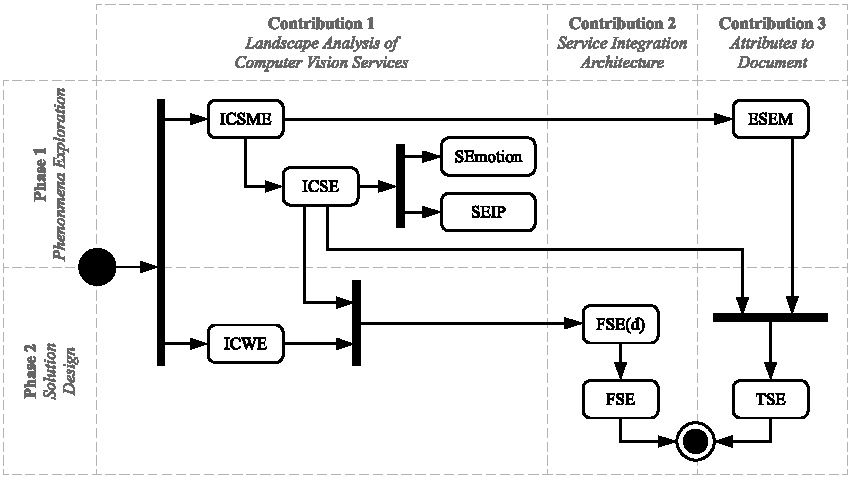
\includegraphics[width=\linewidth]{publications-overview}
  \caption[Overview publication coherency]{Activity diagram of the coherency of our publications, how our research was conducted, and relevant connections between publications. Our two-phase structure initial phenomena exploration and a proposed solutions to issues identified from the exploration. We map the contributions within each publication to the three primary contributions of the thesis.}
  \label{fig:introduction:structure:publications-overview}
\end{figure}

\subsection{Contribution 1: Landscape Analysis \& Preliminary Solutions}

The first two bodies of work in this paper are the ICSME and ICWE papers. These two works investigated a landscape analysis \glspl{cvs} from two perspectives: firstly, we conducted a longitudinal study to better understand the attributes associated with these services (ICSME)---particularly their evolution and behavioural profiles, and their potential impacts to software reliability---and tackled a preliminary solution facade to `merge' responses of the services together (ICWE). 

The ICSME paper confirmed our hypotheses that the services have a non-deterministic behavioural profile, and that the evolution occurring within the \gls{ml} models powering these services are not sufficiently communicated to software engineers. This therefore led to follow up investigation into how developers perceive these services, and thereby determine if they are frustrated due to this lack of communication. 

Our ICWE paper explored one aspect identified from the ICSME paper that we identified early on: that different services use different vocabularies to describe semantically similar objects but in different ways (e.g., `border collie' vs. `collie'), despite offering functionally similar capabilities. We attempted to merge the response labels from these services using a proportional representation approach, and upon comparison with more naive merge approaches, we improved label-merge performance by an F-measure of 0.015. However, while this was an interesting outcome for a preliminary solution design, investigation from our following work suggested that standardising ontologies between service providers becomes challenging and normalising the entire ontological hierarchy of response labels would need to fall under the responsibility of a certain body (that does not exist). Further, we did not find sufficient evidence that developers would frequently switch between service providers. Therefore, we opted for a shielded relay architecture in our later design work.  

\subsection{Contribution 2: Improving Documentation Attributes}

As mentioned, our ICSME paper found that evolutionary and non-deterministic behavioural profile of are not adequately documented in the service's \glspl{api} documentation. A recommendation concluding from this work was that service providers should improve their documentation, however there lacked a strategy by which they could do this, and our hypotheses that developers were actually frustrated by this lack of communication was yet to be tested. This led to two follow-up further investigations as presented in our ICSE and ESEM papers.

One aspect of our ICSE paper was to confirm whether developers are actually frustrated with the service's limited \gls{api} documentation. By mining \glslong{so} posts with reference to documentation issues, we adopted a \citeyear{Aghajani:2019bo} documentation-related taxonomy by \citet{Aghajani:2018et} to classify posts, and found that 47.87\% of posts classified fell under the `completeness' dimension of \citeauthor{Aghajani:2018et}'s taxonomy. This interpretation, therefore, warranted the recommendation proposed in the ICSME paper to improve service documentation. 

However, though improvements to more complete documentation was justified from the ICSE paper, we needed to explore exactly \textit{what} makes a `complete' \gls{api} document. By conducting a \glslong{sms} resulting in 4,501 results, we curated 21 primary studies that outline the facets of \gls{api} documentation knowledge. From these studies, we distilled a documentation framework describing a prioritised order of the documentation assets \gls{api}'s should document that is described in our ESEM short paper. After receiving community feedback, we extended this short paper with a follow-up experiment submitted to TSE. By conducting a survey with developers, we assessed our \gls{api} documentation taxonomy's efficacy with practitioner opinions, thereby producing a weighted taxonomy against \textit{both} literature and developer sources. Lastly, we triangulated both weightings against a heuristic evaluation against common \gls{cvs} providers' documentation. This allowed us to deduce which specific areas in existing \gls{cvs} providers' \gls{api} documentation needed improvement, which was a primary contribution from our TSE article.

\subsection{Contribution 3: Service Integration Architecture}

Two recommendations from our ICSME study encouraged developers to test their applications with a representative ontology for their problem domain and to incorporate a specialised testing and monitoring techniques into their workflow. Strategies on \textit{how} to achieve this were explored in later studies.  Following a similar approach to our solution of improved \gls{api} documentation, we validated the substantiveness of our recommendations using our mining study of \glslong{so} (our ICSE paper) to help inform us of generalised issues developers face whilst integrating \glspl{cvs} into their applications. To achieve this, we used a \glslong{so} post classification taxonomy proposed by \citet{Beyer:2018fm} into seven categories, where 28.9\% and 20.37\% of posts asked issues regarding how to use the \gls{cvs} \gls{api} and conceptual issues behind \glspl{cvs}, respectively. Developers presented an insufficient understanding of the non-deterministic runtime behaviour, functional capability, and limitations of these services and are not aware of key \glslong{cv} terminology. When contrasted to more conventional domains such as mobile-app development, the spread of these issues vary substantially.

We proposed two technical solutions in our two FSE papers to help alleviate this issue. Firstly, our FSE demonstrations paper---FSE(d) for short---provides a workflow for developers to better select an appropriate confidence threshold, and thus decision boundary, calibrated for their particular use case. In our ESEC/FSE paper, we provide a reference architecture for developers to guard against the non-deterministic issues that may `leak' into their applications. This architecture tactic proposes a client-server intermediary proxy server, similar to the style proposed in our ICWE paper. However, unlike the ICWE paper that uses proportional representation approach to modify multiple sources, our FSE paper proposes a guarded relay, whereby a single service is used, and the proxy server maintains a lifecycle to monitor evolution issues identified in ICSME and should be benchmarked against the developer's dataset (i.e., against the particular application domain) as suggested in FSE(d). \todo[For robust component composition, this architecture tactic handles four key requirements: (i) it clearly defines erroneous conditions that occur when evolution occurs in \glspl{cvs}; (ii) it notifies of behavioural changes in the service; (iii) it monitors the service for change and substantial impact this may have to the client application; and (iv) is flexible enough to be implemented and adaptable to any client application or specific intelligent service to facilitate reuse. Both FSE papers serve as two primary contributions to \ref{rq:design}.]{AC: Revised this text.}

% RQ3.3 -- range is diff == existing strategies are not enough!